\documentclass[a4paper]{article}
\usepackage[margin=1in]{geometry}
\usepackage{graphicx}
  \setkeys{Gin}{width=\textwidth, keepaspectratio}
\usepackage{bera}

\renewcommand{\topfraction}{0.5}
\renewcommand{\bottomfraction}{0.9}

\title{CE3115 Experiment G4A---Slope Design}
\author{Mohanadas Harish Chandar (U067314J)}

\begin{document}
\maketitle


\section{Introduction}

A back-analysis of a slope failure was conducted for the client Department of Civil Engineering, National University of Singapore. 

Conditions just after the slope was cut were analysed using undrained parameters. The long term conditions of the slope were analysed using drained parameters with varying water table conditions.

This report outlines the key findings.


\section{Results}
Please see the attached Figures~\ref{fig:undrained}~and~\ref{fig:drained}.


\section{Analysis and Discussion}

\subsection{Causes of slope failure}
The undrained analysis (see Figure~\ref{fig:undrained}) revealed that in the short term the safety factor was above 1. Thus, it did not fail. However, the safety factor was below 1.3 and thus it did not meet the design requirements. 

The slope failed in the long term as the safety factor become less than 1. 
This was found to be the case for several different water table 
conditions. Figure \ref{fig:drained} shows one such condition.

The mechanism of failure is as follows.
Due to unloading because of excavation, pore water pressure increased 
over time. This lead to reduced effective stress and thus reduced shear 
strength in the soil. 
Reduced shear strength in turn lead to reduced maximum resisting moments.
Failure occured when the maximum resisting moment for the failure surface
could no longer overcome the disturbing moment.


\subsection{Improving slope stability}

For long term excavations, the safety factor needs to be above 1.5. Several measures can be taken to achieve this:

\begin{itemize}
\item Reduction of slope gradient
\item Inclusion of a backfill in front of the slope
\item Installation of permanent retaining structures
\item Installation of soil anchors to reach beyond the slip surface
\end{itemize}

A proposed slope with increased stability is given in 
Figure~\ref{fig:drained_modified}. 
It utilises a reduced slope gradient and a backfill in front of the slope.


\section{Conclusion}

It was found that the slope failed in the long term due to the safety factor being less than 1.

A reduced slope gradient, and a backfill in front of the slope were utilised
in designing a slope with increased stability. 


\section*{Figures}

\begin{center}
\begin{figure}[ht]
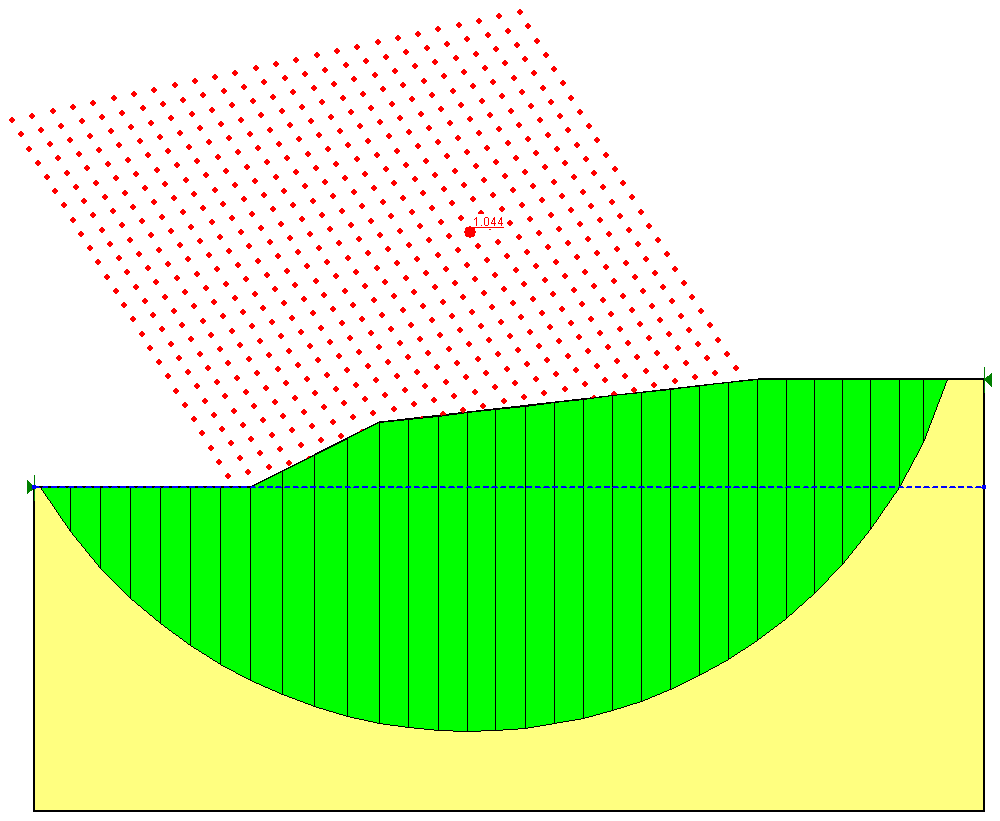
\includegraphics{undrained}
\caption{Conditions just after slope was cut. Safety factor is above 1 but still below design requirement of 1.3.}
\label{fig:undrained}
\end{figure}

\begin{figure}[ht]
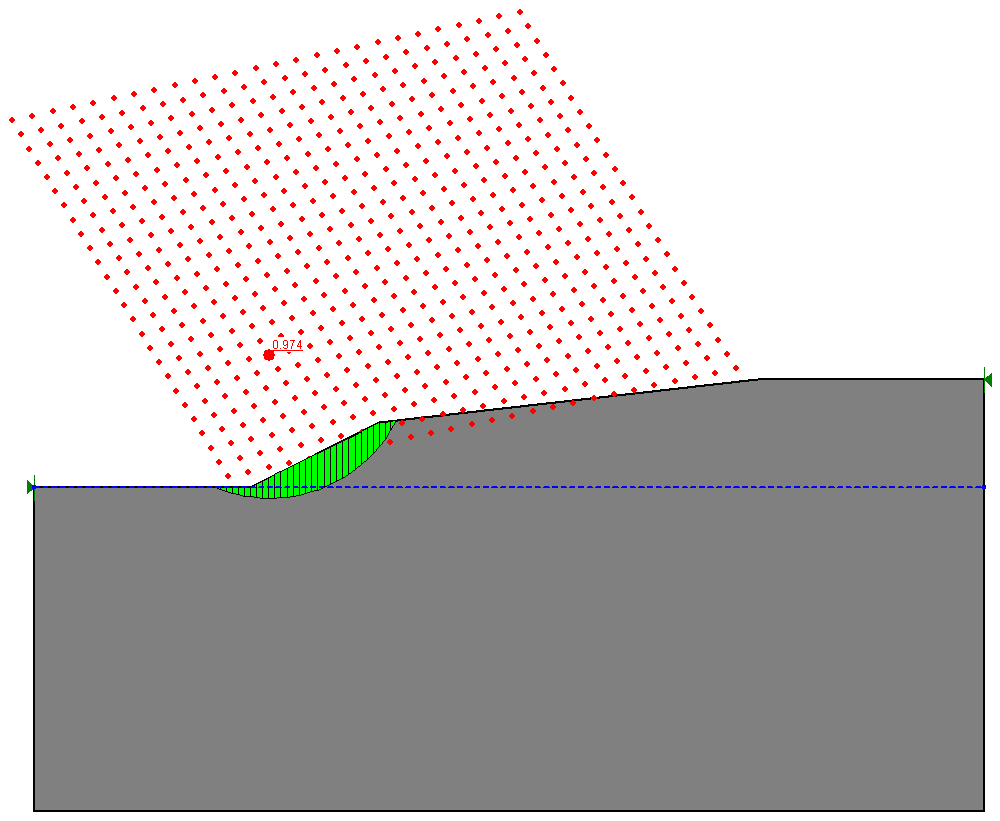
\includegraphics{drained}
\caption{Conditions at slope failure for one of the water table condition. Failure occurs as safety factor is below 1.}
\label{fig:drained}
\end{figure}

\begin{figure}[ht]
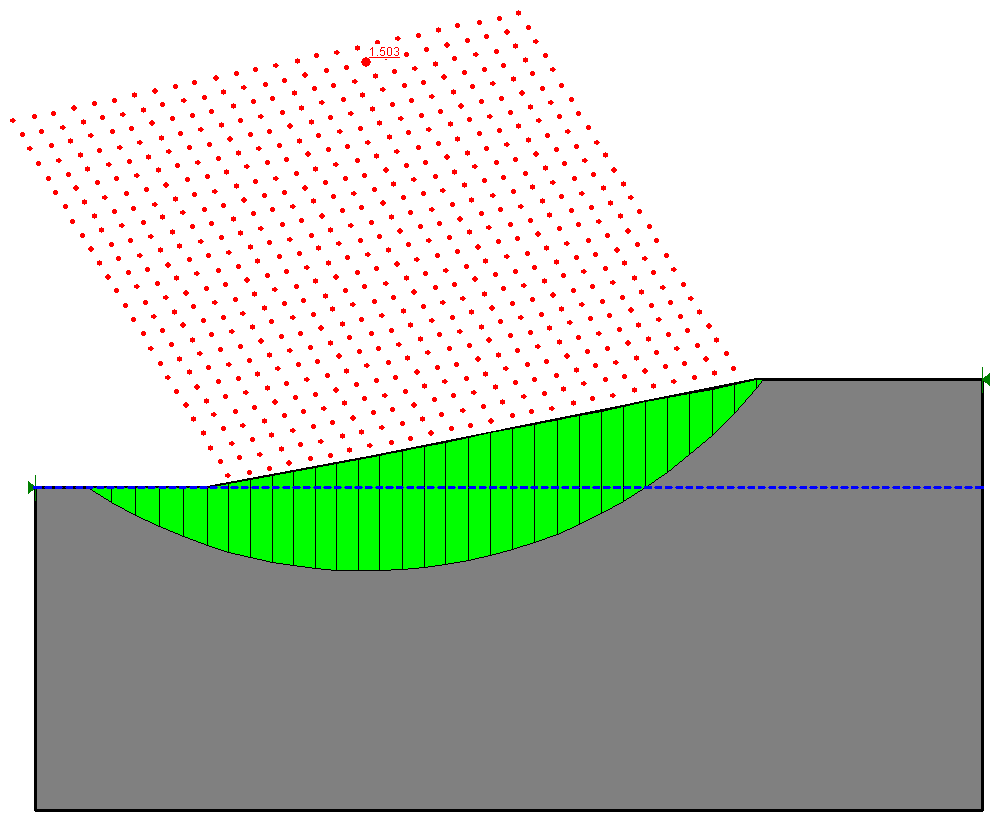
\includegraphics{drained_modified}
\caption{Improved slope design satisfying long term design criteria.}
\label{fig:drained_modified}
\end{figure}
\end{center}


\end{document}
